%##################################################
% Introduction
%##################################################
\section{Introduction}
\subsection{Standard model}

\begin{frame}
    \frametitle{Introduction}

    \centering
    \begin{columns}
        \centering
        \begin{column}{0.5\textwidth}
            \begin{minipage}[c][0.6\textheight][c]{\linewidth}
                \begin{block}{Galaxy groups?}
                    \begin{enumerate}
                        \item<1-> Galaxies reside in groups
                        \item<2-> Result of cosmological formation and baryon
                            physics
                        \item<3-> Still some problems in the scenario
                    \end{enumerate}
                \end{block}
            \end{minipage}
        \end{column}
        \begin{column}{0.5\textwidth}
            \begin{minipage}[c][0.6\textheight][c]{\linewidth}
                \smoothpic[width=\linewidth]{cluster.jpg}
            \end{minipage}
        \end{column}
    \end{columns}
\end{frame}

\begin{frame}
    \frametitle{Introduction}
    \begin{columns}
        \begin{column}{0.5\textwidth}
            \begin{block}{Galaxy formation}
                \begin{enumerate}
                    \item<1-> Dark matter halos grow from initial perturbations
                        in matter density
                    \item<2-> Gas fall into potential well by cooling
                    \item<3-> Heating processes avoid the formation of too
                        massive galaxies
                \end{enumerate}
            \end{block}
        \end{column}
        \begin{column}{0.5\textwidth}
            \begin{minipage}[c][0.6\textheight][c]{\linewidth}
                \only<1>{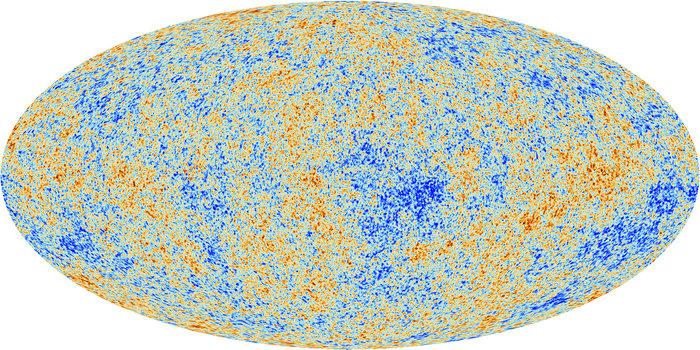
\includegraphics[width=\linewidth]{cmb.jpg}}
                \only<2>{\smoothpic[width=\linewidth]{structures.jpg}}
                \only<3>{\smoothpic[width=\linewidth]{galaxy.jpg}}
            \end{minipage}
        \end{column}
    \end{columns}
\end{frame}

\begin{frame}
    \frametitle{Introduction}
    \begin{columns}
        \begin{column}{0.5\textwidth}
            \begin{block}{Environment modulation}
                \begin{enumerate}
                    \item<1-> Galaxy properties modulated by both local and
                        global environments (morphology, colours, etc)
                    \item<2-> \citet{Peng+11}: specific star formation rate
                        anti-correlates with density for high stellar mass
                        galaxies
                    \item<3-> Consequence of bad quantification of the
                        environment?
                \end{enumerate}
            \end{block}
        \end{column}
        \begin{column}{0.5\textwidth}
            \begin{minipage}[c][0.6\textheight][c]{\linewidth}
                \only<1>{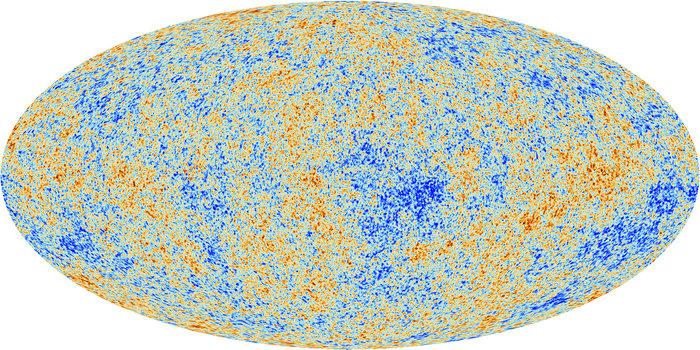
\includegraphics[width=\linewidth]{cmb.jpg}}
                \only<2>{\smoothpic[width=\linewidth]{structures.jpg}}
                \only<3>{\smoothpic[width=\linewidth]{galaxy.jpg}}
            \end{minipage}
        \end{column}
    \end{columns}
\end{frame}

\subsection{Physical processes}

\begin{frame}
    \frametitle{Physical processes}
    \framesubtitle{Mergers}
    \begin{columns}
        \begin{column}{0.5\textwidth}
            \begin{block}{}
                \begin{itemize}
                    \item<1-> Morphologically transform galaxies into
                        spheroidal
                    \item<2-> Bursts of star formation
                \end{itemize}
            \end{block}
        \end{column}
        \begin{column}{0.5\textwidth}
            \smoothpic[width=\linewidth]{merger.jpg}
        \end{column}
    \end{columns}
\end{frame}

\begin{frame}
    \frametitle{Physical processes}
    \framesubtitle{Tidal disruptions}
    \begin{columns}
        \begin{column}{0.5\textwidth}
            \begin{block}{}
                \begin{itemize}
                    \item<1-> Prevents outer gas to be accreted onto galaxy
                        disk
                    \item<2-> Busts of star formation
                \end{itemize}
            \end{block}
        \end{column}
        \begin{column}{0.5\textwidth}
            \smoothpic[width=\linewidth]{tidal.jpg}
        \end{column}
    \end{columns}
\end{frame}

\begin{frame}
    \frametitle{Physical processes}
    \framesubtitle{Harassment}
    \begin{columns}
        \begin{column}{0.5\textwidth}
            \begin{block}{}
                \begin{itemize}
                    \item<1-> Change galaxy morphologies
                    \item<2-> Bursts of star formation
                \end{itemize}
            \end{block}
        \end{column}
        \begin{column}{0.5\textwidth}
            \smoothpic[width=\linewidth]{harassment.jpg}
        \end{column}
    \end{columns}
\end{frame}

\begin{frame}
    \frametitle{Physical processes}
    \framesubtitle{Ram pressure stripping}
    \begin{columns}
        \begin{column}{0.5\textwidth}
            \begin{block}{}
                \begin{itemize}
                    \item<1-> Intra-cluster gas pressure remove gas with low
                        binding to galaxy
                    \item<2-> Quenching of star formation
                \end{itemize}
            \end{block}
        \end{column}
        \begin{column}{0.5\textwidth}
            \smoothpic[width=\linewidth]{rampressure.jpg}
        \end{column}
    \end{columns}
\end{frame}

%##################################################
% Grouping algorithms
%##################################################
\usetikzlibrary{chains,shapes.arrows,fit}
\usetikzlibrary{shadows.blur}

\definecolor{arrowcolor}{RGB}{201,216,232}% color for the arrow filling
\definecolor{circlecolor}{RGB}{79,129,189}% color for the inner circles filling
\colorlet{textcolor}{white}% color for the text inside the circles
\colorlet{bordercolor}{white}% color for the outer border of circles

\pgfdeclarelayer{background}
\pgfsetlayers{background,main}

\newcounter{task}

\newlength\taskwidth% width of the box for the task description
\newlength\taskvsep% vertical distance between the task description and arrow

\setlength\taskwidth{2.5cm}
\setlength\taskvsep{17pt}

\def\taskpos{}
\def\taskanchor{}

\newcommand\task[1]{%
  {\parbox[t]{\taskwidth}{\scriptsize\Centering#1}}}

\tikzset{
inner/.style={
  on chain,
  circle,
  inner sep=4pt,
  fill=circlecolor,
  line width=1.5pt,
  draw=bordercolor,
  text width=1.5em,
  align=center,
  text height=1.25ex,
  text depth=0ex
},
on grid
}

\newcommand\Task[3][]{%
\node[inner xsep=0pt] (c1) {\phantom{A}};
\stepcounter{task}
\ifodd\thetask\relax
  \renewcommand\taskpos{\taskvsep}\renewcommand\taskanchor{south}
\else
  \renewcommand\taskpos{-\taskvsep}\renewcommand\taskanchor{north}
\fi
\node[inner, font=\tiny, #3]
  (c\the\numexpr\value{task}+1\relax) {\color{textcolor}#1};
\node[anchor=\taskanchor,yshift=\taskpos]
  at (c\the\numexpr\value{task}+1\relax) {\task{#2}};
}

\newcommand\drawarrow{% the arrow is placed in the background layer
                                                     % after the node for the tasks have been placed
\ifnum\thetask=0\relax
  \node[on chain] (c1) {}; % if no \Task command is used, the arrow will be drawn
\fi
\node[on chain] (f) {};
\begin{pgfonlayer}{background}
\node[
  inner sep=10pt,
  single arrow,
  single arrow head extend=0.8cm,
  draw=none,
  blur shadow={shadow blur steps=15},
  fill=arrowcolor,
  fit= (c1) (f)
] (arrow) {};
\fill[gray!20!white] % the decoration at the tail of the arrow
  (arrow.before tail) -- (c1|-arrow.west) -- (arrow.after tail) -- cycle;
\end{pgfonlayer}
}

\newenvironment{timeline}[1][node distance=.75\taskwidth]
  {\par\noindent\setcounter{task}{0}\begin{tikzpicture}[start chain,#1]}
  {\drawarrow\end{tikzpicture}\par}

\subsection{Grouping algorithms}
\bartchapterimage{heic9910b_small.jpg}
\bartthumb{thumbs/heic9910b.png}
\renewcommand<>{\tikzset}[1]{\only#2{\beameroriginal{\tikzset}{#1}}}
\tikzset{highlight/.style={fill=green!60!black}}
\tikzset{highlighton1/.style={}}
\tikzset{highlighton2/.style={}}
\tikzset{highlighton3/.style={}}
\tikzset{highlighton4/.style={}}
\begin{frame}
    % \frametitle{Grouping algorithms}
    \begin{minipage}[c][0.29\textheight][c]{\linewidth}
        \begin{timeline}
            \tikzset<1>{highlighton1/.style={highlight}}
            \tikzset<2>{highlighton2/.style={highlight}}
            \tikzset<3>{highlighton3/.style={highlight}}
            \tikzset<4>{highlighton4/.style={highlight}}
            \Task[2002]{Marinoni et al.}{highlighton1}
            \Task[2005]{Yang et al.}{highlighton2}
            \Task[2012]{Dominguez-Romero et al.}{highlighton3}
            \Task[2012]{Munoz-Cuartas et al.}{highlighton4}
        \end{timeline}
    \end{minipage}
    \begin{minipage}[c][0.69\textheight][c]{\linewidth}
        \only<1>{%
            \begin{block}{Marinoni et al. (2002)}
                \begin{minipage}{0.69\linewidth}
                    \begin{enumerate}
                        \item Tessellation of redshift space to estimate
                            over-densities
                    \end{enumerate}
                \end{minipage}
                \begin{minipage}{0.29\linewidth}
                    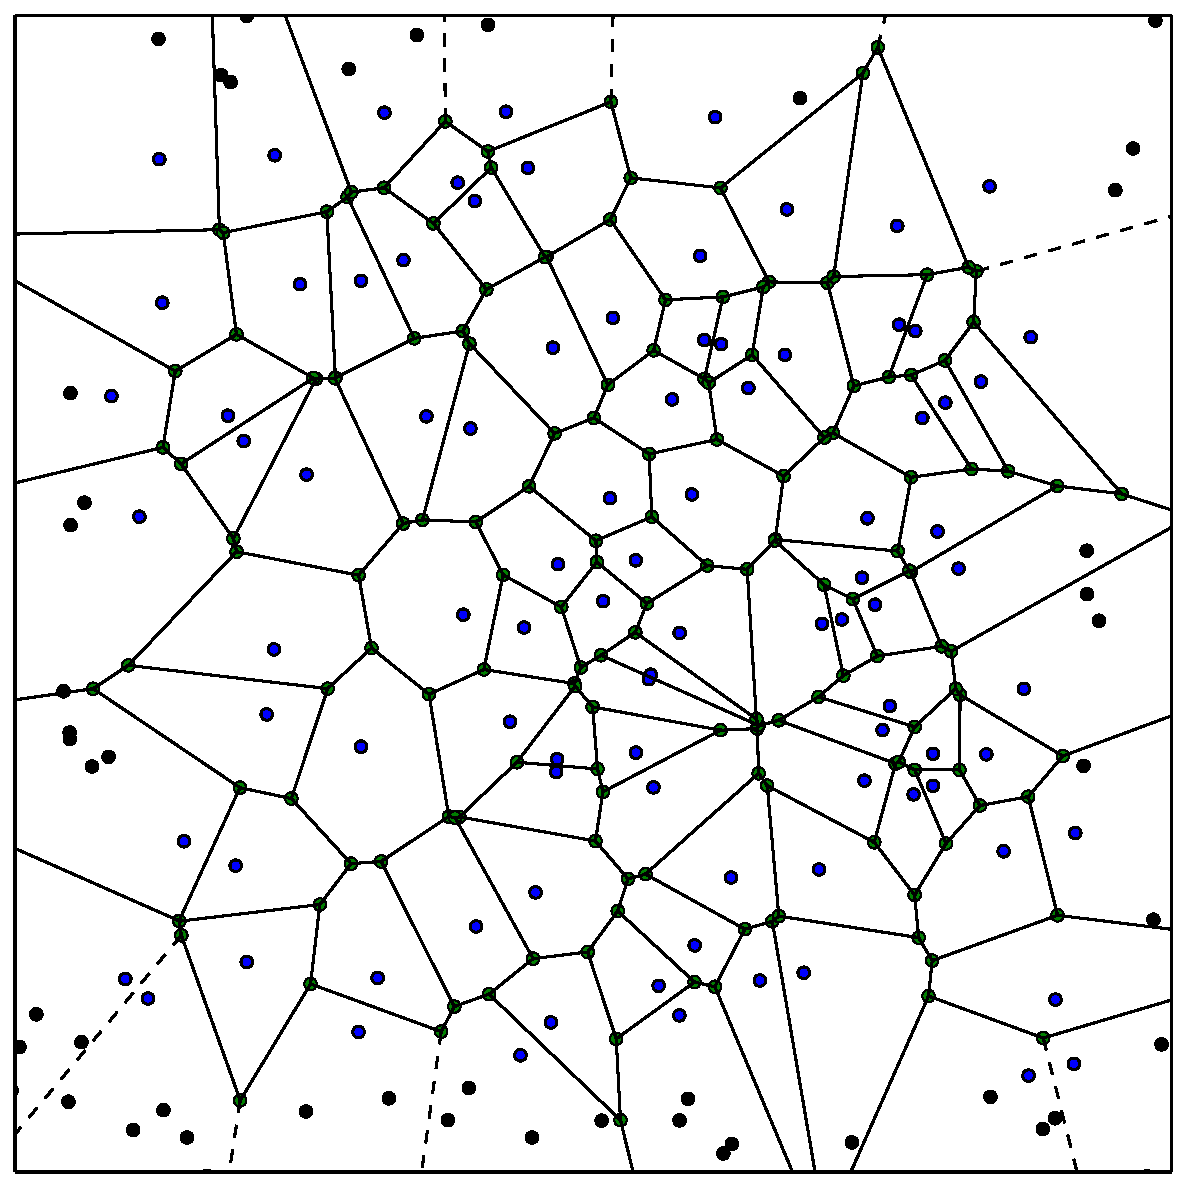
\includegraphics[width=\linewidth]{voronoi.pdf}
                \end{minipage}
            \end{block}
        }
        \only<2>{%
            \begin{minipage}{0.69\linewidth}
                \begin{block}{Yang et al. (2005)}
                    \begin{enumerate}
                        \item Phase space density contrast used as threshold
                            for galaxy assignation to groups
                        \item Iterations for convergence in membership and
                            dynamical mass to light ratio
                        \item Assumes constant interlopers density
                    \end{enumerate}
                \end{block}
            \end{minipage}
        }
        \only<3>{%
            \begin{minipage}{0.69\linewidth}
                \begin{block}{Dominguez Romero et al. (2012)}
                    \begin{enumerate}
                        \item Same as Yang et al.\ but compute responsibilities
                            to belong to a group
                        \item Estimate potential centers by decreasing galaxy
                            stellar masses
                    \end{enumerate}
                \end{block}
            \end{minipage}
        }
        \only<4>{%
            \begin{minipage}{0.69\linewidth}
                \begin{block}{Munoz Cuartas et al. (2012)}
                    \begin{enumerate}
                        \item Kind of FoF applied to halos
                    \end{enumerate}
                \end{block}
            \end{minipage}
        }
    \end{minipage}
\end{frame}

% vim: set tw=79:
